\section{Zielsetzung}
In diesem Versuch soll mittels zweier Scan-Verfahren ein Acrylblock mit Bohrungen vermessen werden (A-Scan und B-Scan).
Wird das Herzschlagvolumen eines Modellherzes gemessen.

\section{Theorie}
Als Ultraschall wird Schall mit einer Frequenz von \SI{20}{\kilo \hertz} bis \SI{1}{\giga \hertz}
beschrieben. Diese Schallfrequenzen kommen in der Medizin in Diagnostik und Therapie zum Einsatz.
Schall ist eine longitudinale Welle, die in einem Medium mittels Druckschwankungen weitergeleitet
wird:
\FloatBarrier
\begin{align*}
  p(x,t) = p_0 + v_0~Z \symup{cos}(\omega t - kx)
\end{align*}
\FloatBarrier
In dieser Gleichung beschreibt $Z$ die akustische Impedanz, welche durch die Dichte $\rho$ und die
Schallgeschwindigkeit $c$ im vorliegenden Stoff beschrieben wird:
\FloatBarrier
\begin{align*}
  Z = c \cdot \rho
\end{align*}
\FloatBarrier
Bei Schallwellen ist die Phasengeschwindigkeit auf Grund von Dichte und Druckschwankungen materialabhängig.
Sie zeigen also im Gegensatz zu elektromagnetischen Wellen Dispersion. Alle anderen grundlegenden
Eigenschaften der elektromagnetischen Wellen zeigen Schallwellen ebenso.
Im Versuch ist lediglich die Schallweiterleitung in Festkörpern von Bedeutung, welche durch
folgenden Zusammenhang zwischen $E$, dem Elastizitätsmodul und der Dichte $\rho$ beschrieben wird:
\FloatBarrier
\begin{align*}
  c_{\symup{\tiny{FK}}} = \sqrt{\frac{E}{\rho}}
\end{align*}
\FloatBarrier
Hierbei ist zu beachten, dass $c_{\symup{\tiny{FK}}}$ für transversale und longitudinale Wellen
unterschiedlich aussieht.
Breiten sich Schallwellen in einem Festkörper aus, so verlieren diese durch Absorption exponentiell an Energie.
Somit wird die Intensität einer Welle durch folgenden Zusammenhang beschrieben:
\FloatBarrier
\begin{align*}
  I(x) = I_0 \cdot \symup{e}^{(-\alpha ~ x)}
\end{align*}
\FloatBarrier
In dieser Gleichung beschreibt $\alpha$ den Absorptionskoeffizienten, $I_0$ die Anfangsintensität und $x$
die zurückgelegte Strecke.
Der Absorptionskoeffizient ist für Luft sehr groß, weshalb im Versuch darauf zu achten ist, dass
stets ein Kontaktmittel zwischen Ultraschallkopf und zu untersuchendem Körper verwendet wird.
Bei dem Kontaktmittel handelt es sich um Hydrogel oder bidestilliertes Wasser.
Treffen Schallwellen auf Grenzflächen, so werden sie reflektiert. Die Reflexion kann durch den
Reflexionskoeffizienten $R$ beschrieben werden, für dessen Berechnung die Impedanzen der beiden
Materialien, die die Grenzfläche bilden, wichtig sind:
\FloatBarrier
\begin{align*}
  R = \left(\frac{Z_1 - Z_2}{Z_1 + Z_2} \right)^2
\end{align*}
\FloatBarrier
Der Reflexionskoeffizient gibt das Verhältnis zwischen einlaufender und reflektierter Welle an.
Folglich ergibt sich der Transmissionskoeffizient zu $T = 1 ~ - R$.
Um Ultraschallwellen zu erzeugen, wird der Piezoelektrische Effekt verwendet, wobei ein piezoelektrischer
Kristall (Quarz) mittels eines elektrischen Feldes in Schwingung versetzt wird, wodurch dieser
Ultraschallwellen emittiert. Das elektrische Feld übt eine Kraft auf die einzelnen Ladungen im Kristallgitter aus,
welches sich daraufhin zusammenzieht oder ausdehnt und somit beginnt zu schwingen. Umgekehrt können Schallwellen
das Kristallgitter in Schwingung versetzen, wodurch sich der Ladungsschwerpunkt verschiebt und folglich eine
Spannung anliegt. So kann der piezoelektrische Effekt ebenso zur Detektion von Ultarschallwellen genutzt werden.
Mittels Ultraschall ist es so möglich Aussagen über die Beschaffenheit von Körpern zu treffen, ohne diese eröffnen
zu müssen.
Dies kann auf zwei verschiedene Arten geschehen. Zum einen, indem von einem Sender ein kurzer Schallimpuls durch das
Medium ausgesendet wird, welcher von einem Detektor auf der anderen Seite des zu utersuchenden Körpers aufgefangen wird.
Mögliche Fehlstellen sind durch eine Abschwächung des Signals zu erkennen. Die Lokalisation dieser ist jedoch nicht möglich.
Dieses Verfahren wird Durchschallungsverfahren genannt und ist schematisch in Abbildung \ref{abb1} zu sehen.
\FloatBarrier
\begin{figure}
  \centering
  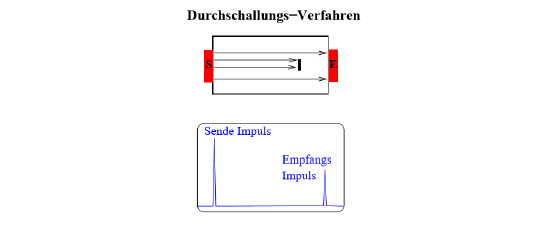
\includegraphics[scale=0.8]{1.PNG}
  \caption{Schematische Darstellung des Durchschallungsverfahrens.\cite{Q1}}
  \label{abb1}
\end{figure}
\FloatBarrier
Das zweite Verfahren, das bei der Unteruschung von Medien zum Einsatz kommt, ist das Impuls-Echo-Verfahren.
Hierbei fungiert der Schallkopf sowohl als Sender als auch als Empfänger, der an den Grenzflächen
emittierten Ultraschallwellen. Wie aus Abbildung \ref{abb2} hervorgeht, ist es mittels dieser Methode möglich,
etwaige Fehlstellen zu detektieren. Deren Größe kann durch die Höhe der gemessenen Reflexion abgeschätzt werden.
Ist die Schallgeschwindigkeit im Medium bekannt, so kann mittels folgender Formel ebenfalls die Lage der
Fehlstelle ermittelt werden:
\FloatBarrier
\begin{align*}
  s = \frac{1}{2} c ~ t
\end{align*}

\FloatBarrier
\begin{figure}
  \centering
  
\includegraphics[scale=0.7]{2.PNG}
  \caption{Schematische Darstellung des Impuls-Echo-Verfahrens. \cite{Q1}}
  \label{abb2}
\end{figure}
\FloatBarrier


\section{Durchführung}
Bevor mit den Scans begonnen wird, muss der Acrylblock mittels einer Schieblehre ausgemessen werden. Der Acrylblock ist schematisch in Abbildung
\ref{abb3} zu sehen.
\begin{figure}
  \centering
  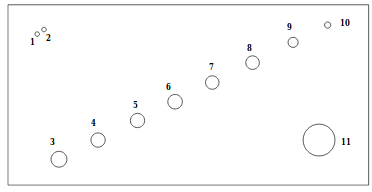
\includegraphics[scale=0.5]{Acrylbox.png}
  \caption{Schematische Ansicht des Acylblockes. \cite{Q1}}
  \label{abb3}
\end{figure}
Im ersten Versuchsteil soll dieser Acrylblock nun mit Hilfe eines A-Scans vermessen werden. Hierzu wird eine \SI{1}{\mega\hertz}-Sonde mit Wasser
auf der Oberseite des Blocks gekoppelt. Um den Abstand der Löcher von der Oberseite des Acrylblocks zu ermitteln, wird die Sonde direkt über das zu
vermessenen Loch gesetzt und ein A-Scan durchgeführt, bei dem die Spannung $U$ gegen die Zeit $t$ aufgetragen wird.
Es wird die Zeit des reflektierten Impulses von dem entstehenden Graphen abgelesen.
Dieses wird für jede einzelne Bohrung durchgeführt. Bei der doppelten Bohrung muss gegebenenfalls der zeitlich spätere Bereich verstärkt werden, um
die Peaks genau abmessen zu können.
Nachdem alle Bohrungen vermessen sind, wird der Block gedreht und das selbe von der anderen Seite durchgeführt.

Im zweiten Teil des Versuchs sollen die Bohrungen 1 und 2 (siehe \ref{abb3}) genauer untersucht werden, da diese durch den ersten Versuchsteil kaum
zu differenzieren sind. Hierzu sollen Bilder eines A-Scans von den Bohrungen 1 und 2 gemacht werden. Zunächst wird ein A-Scan mit einer
\SI{1}{\mega\hertz}-Sonde durchgeführt, wie im vorherigen Versuchsteil. Danach wird eine \SI{2}{\mega\hertz}-Sonde angeschlossen und erneut ein
A-Scan durchgeführt, um beide Bohrungen besser unterscheiden zu können. Auch hier werden die reflektieren Signale für größere Zeiten verstärkt,
um die Peaks besser ablesen zu können.

Der selbe Acrylblock soll im dritten Versuchsteil durch einen B-Scan vermessen werden. Hierzu wird erneut eine \SI{1}{\mega\hertz}-Sonde auf der
Oberseite des Acrylblocks mit Wasser als Verbindungsschicht gekoppelt. Nun wird bei dem Programm auf B-Scan umgestellt und gestartet. Während das
Programm läuft, wird die Sonde langsam über die Oberfläche des Acrylblocks geschoben. Das enstehende Diagramm wird gespeichert.
Auch bei diesem Versuchsteil wird der Block gedreht und es wird erneut ein B-Scan von der Unterseite des Acrylblock durchgeführt.

Im letzten Versuchsteil soll das Herzzeitvolumen eines Herzmodells gemessen werden. Hierzu wird das Herzmodell zu einem Drittel mit
destilliertem Wasser befüllt und eine \SI{1}{\mega\hertz}-Sonde darüber angebracht, sodass diese so eben das Wasser berührt.
Nun wird ein A-Scan durchgeführt und die Zeit des reflektierten Schalls gemessen. Daraufhin wird das Herzmodell mittels eines Gummiballs
aufgepumpt und in diesem Zustand erneut ein A-Scan durchgeführt und die Zeit des reflektierten Schalls gemessen.
Nun wird ein B-Scan des Herzmodells durchgeführt, indem das Herzmodell mittels des Gummiballs periodisch aufgepumpt wird. Dabei
sollten mindestens 5 Herzschläge simuliert werden. Die Frequenz sollte hierbei möglichst konstant bleiben. Zuletzt wird
der Durchmesser des Herzmodells mittels einer Schieblehre bestimmt.
